\documentclass[11pt, a4paper, twoside]{article}   	% use "amsart" instead of "article" for AMSLaTeX format

\usepackage{geometry}                		% See geometry.pdf to learn the layout options. There are lots.
\usepackage{pdfpages}
\usepackage{caption}
\usepackage{minted}
\usepackage[german]{babel}			% this end the next are needed for german umlaute
\usepackage[utf8]{inputenc}
\usepackage{color}
\usepackage{graphicx}
\usepackage{titlesec}
\usepackage{fancyhdr}
\usepackage{lastpage}
\usepackage{hyperref}
\usepackage[autostyle=false, style=english]{csquotes}
\usepackage{mathtools}
\usepackage{tabularx}
% http://www.artofproblemsolving.com/wiki/index.php/LaTeX:Symbols#Operators
% =============================================
% Layout & Colors
% =============================================
\geometry{
   a4paper,
   total={210mm,297mm},
   left=20mm,
   right=20mm,
   top=20mm,
   bottom=30mm
 }	

\definecolor{myred}{rgb}{0.8,0,0}
\definecolor{mygreen}{rgb}{0,0.6,0}
\definecolor{mygray}{rgb}{0.5,0.5,0.5}
\definecolor{mymauve}{rgb}{0.58,0,0.82}

\setcounter{secnumdepth}{4}


% the default java directory structure and the main packages
\newcommand{\scrRoot}{../src/aspectj}
\newcommand{\srcDirTracing}{\scrRoot/tracing/src/main/java}
\newcommand{\srcDirCaching}{\scrRoot/caching/src/main/java}
\newcommand{\srcDirTspSolver}{\scrRoot/tsp-solver/src/main/java}
\newcommand{\imageDir}{images}
% =============================================
% Code Settings
% =============================================
\newenvironment{code}{\captionsetup{type=listing}}{}
\newmintedfile[javaFile]{java}{
	linenos=true, 
	frame=single, 
	breaklines=true, 
	tabsize=2,
	numbersep=5pt,
	xleftmargin=10pt,
	baselinestretch=1,
	fontsize=\footnotesize
}

\newcommand{\xvdash}[1]{%
  \vdash^{\mkern-10mu\scriptscriptstyle\rule[-.9ex]{0pt}{0pt}#1}%
}

% =============================================
% Page Style, Footers & Headers, Title
% =============================================
\title{Übung 3}
\author{Thomas Herzog}

\lhead{Übung 3}
\chead{}
\rhead{
\includegraphics[scale=0.10]{FHO_Logo_Students.jpg}}

\lfoot{S1610454013}
\cfoot{}
\rfoot{ \thepage / \pageref{LastPage} }
\renewcommand{\footrulewidth}{0.4pt}
% =============================================
% D O C U M E N T     C O N T E N T
% =============================================
% =============================================
% 2016.10.13: 1 
% 2016.10.14: 2
% =============================================
\pagestyle{fancy}
\begin{document}
\setlength{\headheight}{15mm}
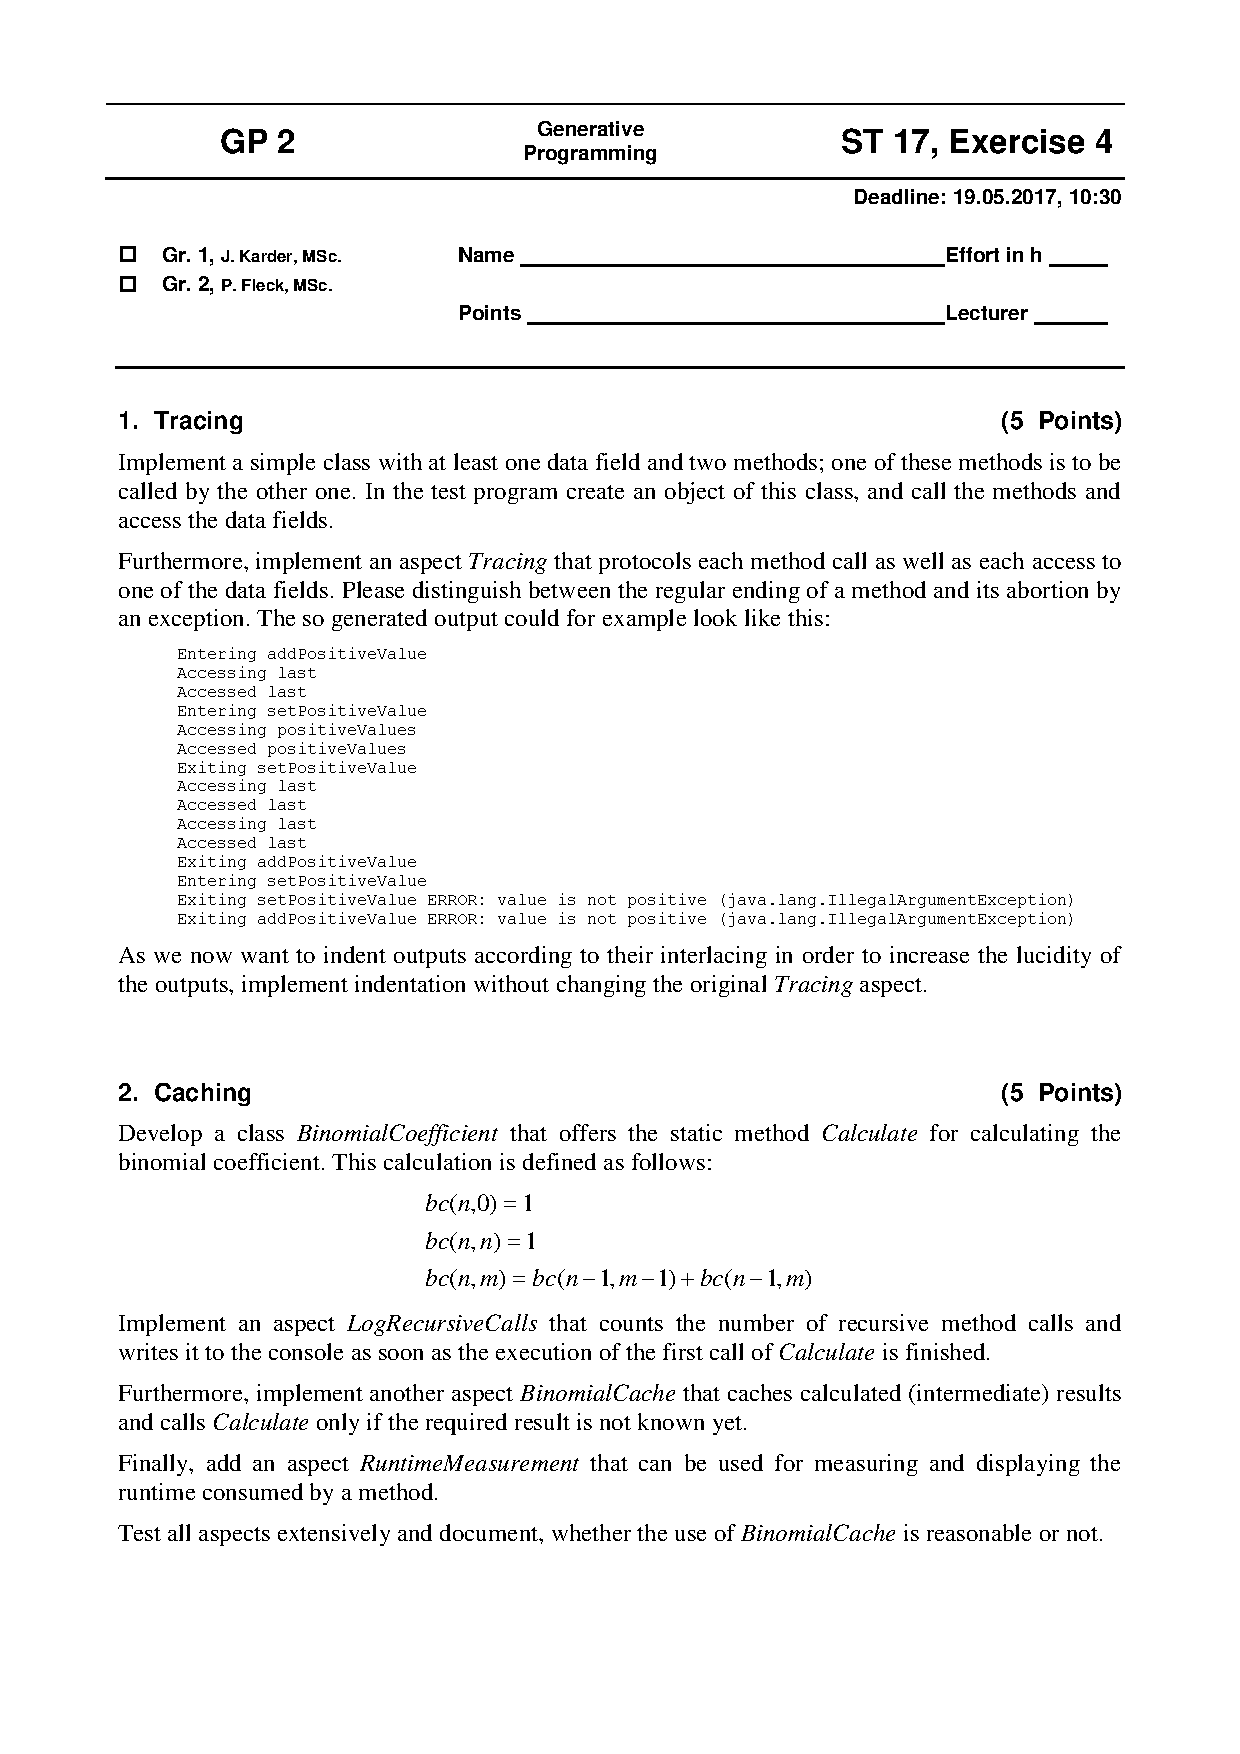
\includepdf[pages={1,2}]{GP_A04.pdf}

\section{Tracing}
Dieser Abschnitt beschäftigt sich mit der Dokumentation der Aufgabenstellung \emph{Tracing}.
\subsection{Lösungsidee} 
Für das Testen des \emph{tracing} \emph{application.PositiveValueStore} implementiert, die mehrere verschachtelte Aufrufe sowie das Auslösen einer Ausnahme simuliert. Die Klasse \emph{application.Main} wurde von en Aspekten ausgenommen, damit die implementierten Testmethoden nicht in den \emph{Logs} aufscheinen.
\newline
\newline
Der Aspekt \emph{TracingAspect} \emph{traced} alle Konstruktoraufrufe, Methodenaufrufe und Parameterzugriffe von Klassen bevor und nachdem Zugriff. Als \emph{Loggingframework} wird \emph{slf4j} verwendet. Alle Zugriffe werden in die Logdatei \emph{aspectj/logs/tracing-logfile.txt} geschrieben.
\newline
\newline
Der Aspekt \emph{IndentionLogTrace} realisiert das Einrücken der logs um die Verschachtelung der Methodenaufrufe zu verdeutlichen. Es wird ein \emph{Pointcut} auf alle Methoden der Schnittstelle \emph{org.slf4j.Logger} definiert, und ein \emph{Around Advice} implementiert der den übergebenen Text formatiert, je nachdem ob eine erwarteter Zeichenkette (\emph{Before method, After method, Before constructor, After constructor}) am Anfang des Textes gefunden wurde. Wird eine solche Zeichenkette am Anfang des Textes gefunden wird bei \emph{Before ...} eine definierte Anzahl von Leerzeichen am Anfang des Textes eingefügt und beim Finden des Textes \emph{After ...} einmalig die definierte Anzahl von Leerzeichen am Anfang des Textes entfernt.

\subsection{Quelltexte}
Folgender Abschnitt enthält die implementierten Klassen, Aspekte und das implementierte Testprogramm.
\begin{code}
	\caption{PositiveValueStore.java}
	\javaFile{\srcDirTracing/application/PositiveValueStore.java}
	\label{src:class-positive-value-store}
\end{code}

\begin{code}
	\caption{TracingAspect.aj}
	\javaFile{\srcDirTracing/aspects/TracingAspect.aj}
	\label{src:aspect-tracing}
\end{code}

\begin{code}
	\caption{IndentionLogTrace.aj}
	\javaFile{\srcDirTracing/aspects/IndentionLogTrace.aj}
	\label{src:aspect-indention-log-trace}
\end{code}

\begin{code}
	\caption{Main.java}
	\javaFile{\srcDirTracing/application/Main.java}
	\label{src:class-tracing-main}
\end{code}

\subsection{Tests}
Folgender Abschnitt enthält die Tests der Aufgabenstellung in Form der generierten \emph{logs}

\begin{figure}[h]
	\centering
	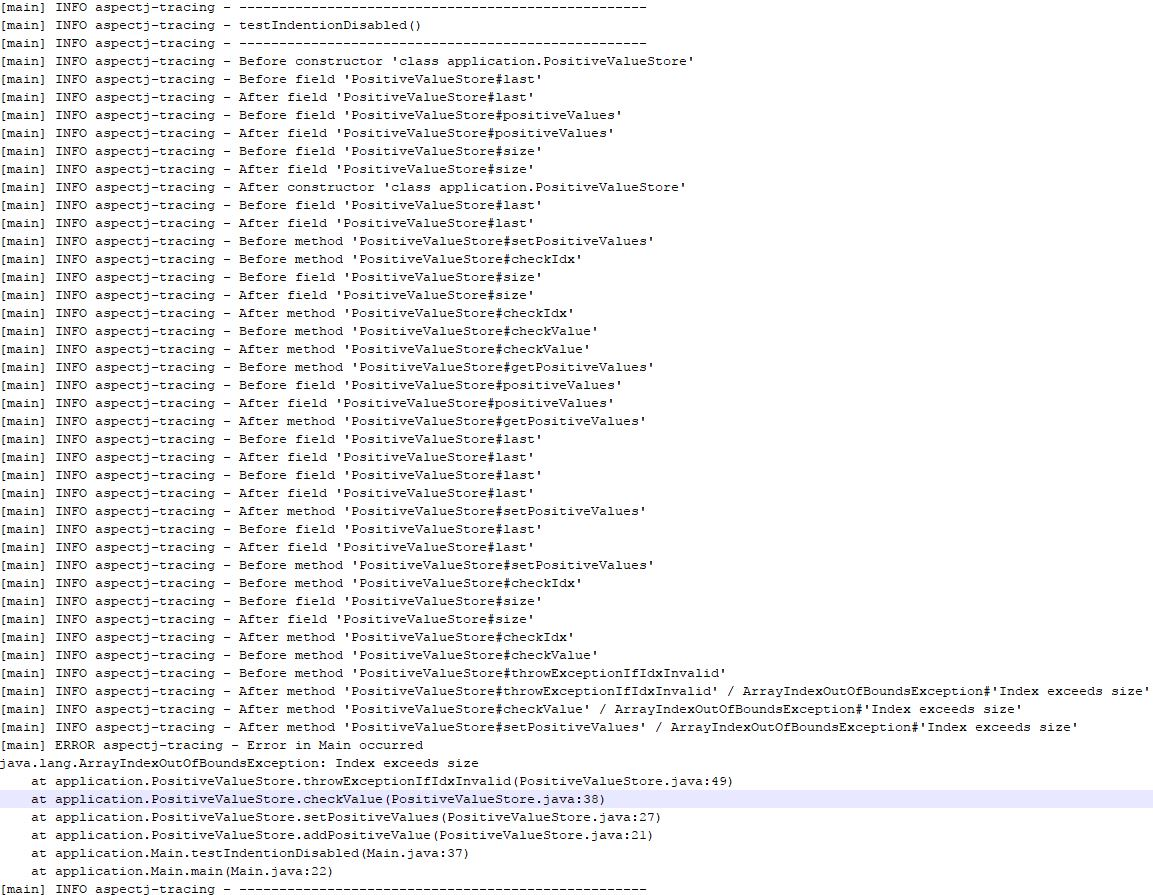
\includegraphics[scale=0.5]{\imageDir/tracing-non-indention-log.JPG}
	\caption{Nicht eingerückter \emph{log}}
	\label{fig:tracing-non-indention-log}
\end{figure}
\ \newpage
\begin{figure}
	\centering
	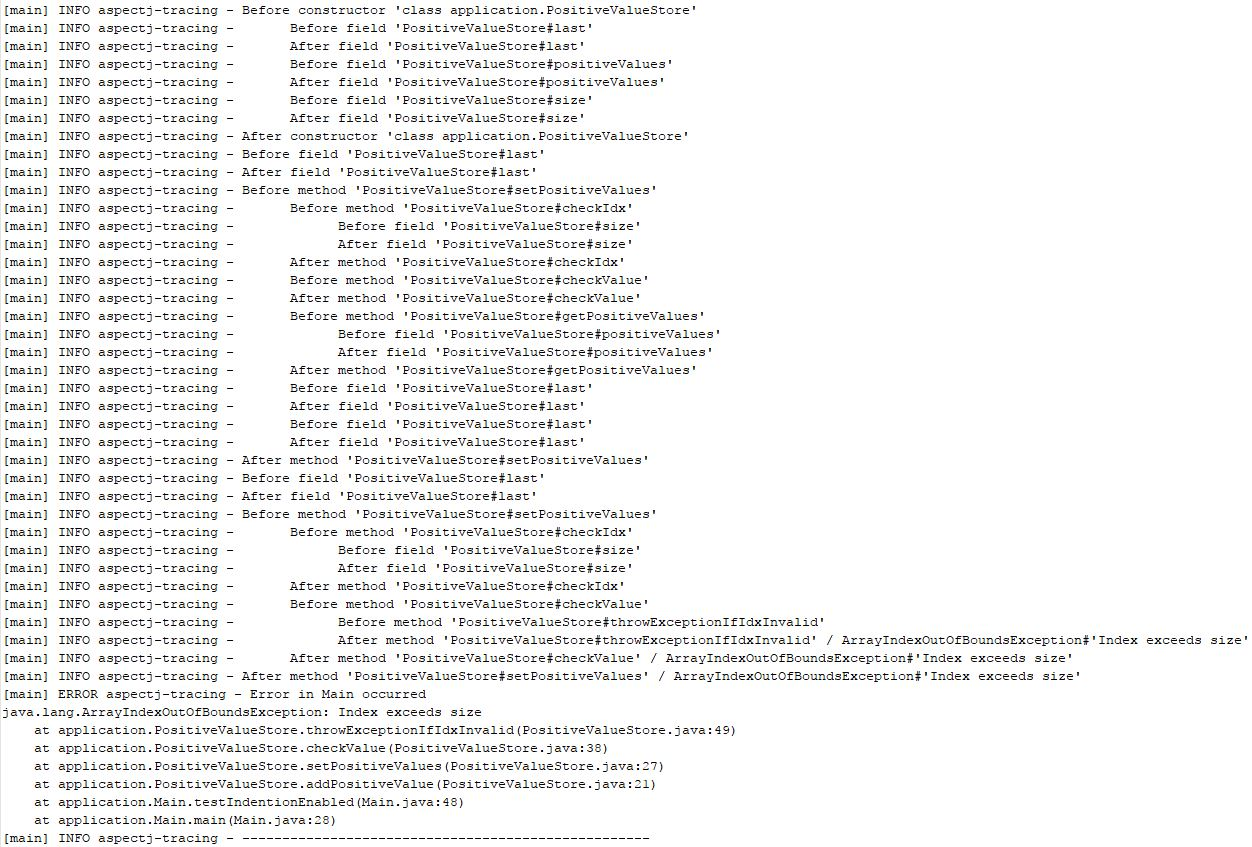
\includegraphics[scale=0.5]{\imageDir/tracing-indention-log.JPG}
	\caption{Eingerückter \emph{log}}
	\label{fig:tracing-indention-log}
\end{figure}
\ \newpage

\section{Caching}
Dieser Abschnitt beschäftigt sich mit der Dokumentation der Aufgabenstellung \emph{Caching}.

\subsection{Lösungsidee} 
Der Algorithmus für die Berechnung des Binominialkoeffizienten wird in der Klasse \emph{BinomialCoefficient} implementiert.
\newline
\newline
Es wird ein abstrakter Aspekt \emph{AbstractAspect} implementiert, der die \emph{Pointcut} \emph{firstCall}, \emph{allCallsWithArgs} und \emph{innerCalls} definiert, sowie \emph{Advices} für \emph{firstCall}, die abstrakte Methoden aufrufen. Dies soll so strukturiert werden, da alle Aspekte auf den ersten Aufruf der Berechnungsmethode reagieren sollen, um ihre Zustände zu initialisieren und zurückzusetzen. Dazu werden zwei Methoden \emph{beforeFristCall} und \emph{afterFirstCall} zur Verfügung gestellt, die von den konkreten Aspekten überschrieben werden können. Die Methoden \emph{beforeFristCall} und \emph{afterFirstCall} sind mit leeren Methodenrumpf in der Klasse \emph{AbstractAspect} implementiert. 
\newline
\newline
Es wird der Aspekt \emph{LogRecursiveCallsAspect} implementiert, der einen \emph{Advice} definiert, der nur ausgeführt wird wenn das \emph{Logging} aktiviert wurde und die Bedingungen definiert im \emph{PointCut innerCalls} erfüllt sind. Beim ersten Aufruf der Berechnungsmethode wird vor dem Aufruf der Methode der Zähler initialisiert und nach dem Aufruf das Resultat über den \emph{Logger} in die \emph{Logs} geschrieben und der Zähler wieder zurückgesetzt.
\newline
\newline
Es wird der Aspekt \emph{BinomialCacheAspect} implementiert, der die Berechnungsergebnisse zwischenspeichert um sie bei einem erneuten Auftreten der Variablen \emph{n, m} zurückliefert und so einen weiteren rekursiven Abstiegt verhindert. Es wird die Klasse \emph{BinomMapKey} implementiert, die als Schlüssel in einer \emph{java.util.HashMap} fungiert, die wiederum die berechneten Werte speichert. Das Zwischenspeichern wird nur dann durchgeführt, wenn \emph{Main.CachingEnabled} auf den Wert \emph{true} gesetzt ist.
\newline
\newline
Es wird der Aspekt \emph{RuntimeMeasurementAspect} implementiert, der die Dauer der gesamten Berechnung misst und über den \emph{Logger} ind \emph{Logs} schreibt. Das Messen der Zeit wird nur dann durchgeführt wenn \emph{Main.LoggingEnabled} auf den Wert \emph{true} gesetzt ist.

\subsection{Quelltexte}
Folgender Abschnitt enthält die implementierten Klassen, Aspekte und das implementierte Testprogramm.

\begin{code}
	\caption{AbstractAspect.aj}
	\javaFile{\srcDirCaching/aspects/AbstractAspect.aj}
	\label{src:class-caching-abstract-aspect}
\end{code}

\begin{code}
	\caption{LogRecursiveCallsAspect.aj}
	\javaFile{\srcDirCaching/aspects/LogRecursiveCallsAspect.aj}
	\label{src:class-caching-log-recursive-calls-aspect}
\end{code}

\begin{code}
	\caption{BinomialCacheAspect.aj}
	\javaFile{\srcDirCaching/aspects/BinomialCacheAspect.aj}
	\label{src:class-caching-log-cache-aspect}
\end{code}

\begin{code}
	\caption{RuntimeMeasureAspect.aj}
	\javaFile{\srcDirCaching/aspects/RuntimeMeasureAspect.aj}
	\label{src:class-caching-runtime-measurement-aspect}
\end{code}

\begin{code}
	\caption{BinomMapKey.java}
	\javaFile{\srcDirCaching/model/BinomMapKey.java}
	\label{src:class-caching-binom-map-key}
\end{code}

\begin{code}
	\caption{BinomialCoefficient.java}
	\javaFile{\srcDirCaching/application/BinomialCoefficient.java}
	\label{src:class-caching-class-binom}
\end{code}

\begin{code}
	\caption{Main.java}
	\javaFile{\srcDirCaching/application/Main.java}
	\label{src:class-caching-class-binom}
\end{code}

\subsubsection{Tests}
Folgender Abschnitt enthält die Tests der Aufgabenstellung in Form der generierten \emph{logs}.
\newline
\newline
Während der Tests hat sich gezeigt, das mit aktiviertem \emph{Caching} sich das Laufzeitverhalten deutlich verbessert hat, da die rekursiven Aufrufe deutlich weniger geworden sind und daher auch die Anzahl der Berechnungen sich deutlich verringert hat.

\begin{figure}[h]
	\centering
	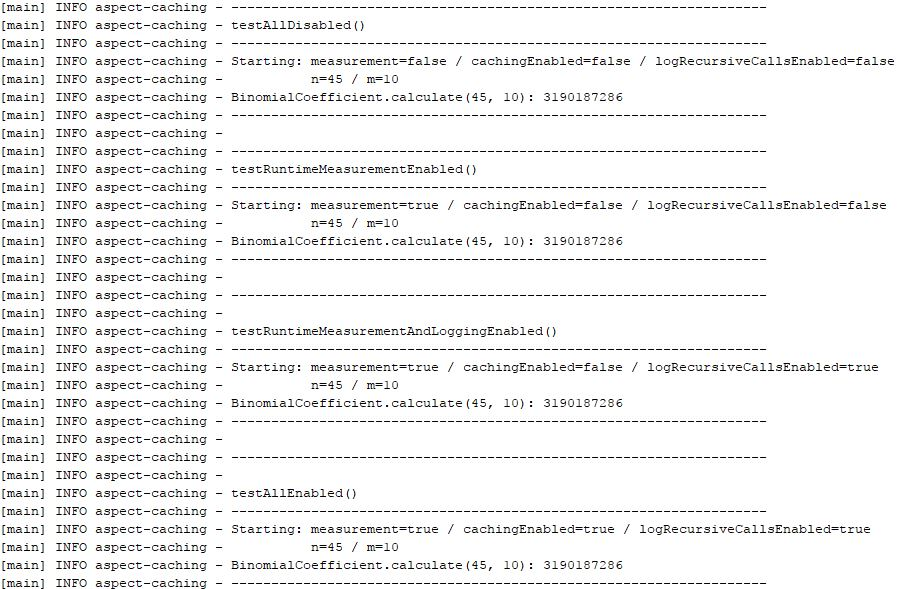
\includegraphics[scale=0.7]{\imageDir/caching-log.JPG}
	\caption{\emph{Caching} Test \emph{Logs}}
	\label{fig:caching-log}
\end{figure}
\ \newpage

\section{Asepct-Oriented TSP Solver}
Dieser Abschnitt beschäftigt sich mit der Dokumentation der Aufgabenstellung \emph{Asepct-Oriented TSP Solver}.
\subsection{Lösungsidee}
Die Projektstruktur wurde dahingehend verändert, dass die Schnittstellen und die \emph{Exceptions} in eigene Pakete ausgelagert wurden. Die Konfiguration der Aspekte wurde in der Klasse \emph{util.AspectjConfig} zusammengeführt, die jetzt alle booleschen Variablen enthält die von den Aspekten verwendet werden, um zu entscheiden, ob sie aktiviert sind oder nicht. Die nötigen Änderungen in den bestehenden Aspekten wurden vorgenommen, damit die Aspekte mit der geänderten Projektkonfiguration arbeiten können.
\newline
\newline
Es wird der Aspekt \emph{CountEvaluatedSolutionsAspect} implementiert, der die Anzahl der evaluierten Lösungen zählt. Es wird ein \emph{PointCut executeCall} definiert, auf den die beiden \emph{before advice, after advivce} hängen, wobei der \emph{before advice} vor dem Methodenaufruf der Methode \emph{Algorithm.execute} den Zähler initialisiert der \emph{after advice} nach dem Methodenaufruf der Methode \emph{Algorithm.execute} das Resultat über einen \emph{Logger} in die \emph{Logs} schreibt und den Zähler zurücksetzt. Ein weiterer \emph{after advice} erhöht den Zähler nach dem Methodenaufruf der Methode \emph{Solution.evaluate}. Dieser Aspekt arbeitet nur gegen die Schnittstellen \emph{Algorithm} und \emph{Solution} und ist daher auf alle Implementierungen dieser Schnittstellen anwendbar. Dieser Aspekt greift nur wenn die Variable \emph{AspectjConfig.countSolutionsEnabled} auf den Wert \emph{true} gesetzt ist.
\newline
\newline
Es wird der Aspekt \emph{GAElitismAspect} implementiert, der die schlechteste Lösung der neu erstellten Kinder durch die beste Lösung des vorherigen Durchlaufs ersetzt. Es wird ein \emph{around advice} für die Methode \emph{GA.createChildren} implementiert, der das zurückgelieferte \emph{Array} der Kinder verändert. Wird ein Kind ausgetauscht so wird eine Meldung über einen \emph{Logger} in die \emph{Logs} geschrieben. Dieser Aspekt ist abhängig von der Klasse \emph{GA}, da die Schnittstelle \emph{Algorithm} die Methode \emph{createChildren} nicht definiert. Dieser Aspekt greift nur wenn die Variable \emph{AspectjConfig.elitismEnabled} auf den Wert \emph{true} gesetzt ist.
\newline
\newline
Es wird der Aspekt \emph{GAProtocolProgressAspect} implementiert, der die beste Lösung, schlechteste Lösung und den Durchschnitt der Lösungen einer Population einer Iteration speichert und nach dem Ausführen des Algorithmus über einen \emph{Logger} in die \emph{Logs} schreibt und ein SVG-Diagramm mit der Bibliothek \emph{gp2.svg-generator} erstellt. Es wird der \emph{PointCut firstExecuteCall} definiert, für den die beiden \emph{advices before, after} definiert werden, wobei der \emph{advice before} die Zustände des Aspekts initialisiert und der \emph{advice after} die Zustände des Aspekts zurücksetzt. Es werden zwei \emph{after advices} definiert, wobei ein \emph{after advice} nach der Ausführung der Methode \emph{Algorithm.initialize} und der andere \emph{after advice} nach der Ausführung der Methode \emph{Algorithm.iterate} greift. Der \emph{after advice} für die Methode \emph{Algorithm.initialize} ist notwendig, weil dort die erste Population erstellt wird. Dieser Aspekt greift nur wenn die Variable \emph{AspectjConfig.reportAlgorithmEnabled} auf den Wert \emph{true} gesetzt ist.
\newline
\newline
Es wird eine Klasse \emph{AspectReport} implementiert, welche die gesammelten Daten einerseits über einen \emph{Logger} in die \emph{Logs} schreibt und andererseits ein SVG-Diagramm erstellt. 
\newpage

\subsection{Quelltexte}
Folgender Abschnitt enthält die implementierten Klassen, Aspekte und das implementierte Testprogramm.

\begin{code}
	\caption{CountEvaluatedSolutionsAspect.aj}
	\javaFile{\srcDirTspSolver/aspects/CountEvaluatedSolutionsAspect.aj}
	\label{src:class-tsp-solver-count-eval-aspect}
\end{code}

\begin{code}
	\caption{GAElitismAspect.aj}
	\javaFile{\srcDirTspSolver/aspects/GAElitismAspect.aj}
	\label{src:class-tsp-solver-ga-elitism-aspect}
\end{code}

\begin{code}
	\caption{GAProtocolProgressAspect.aj}
	\javaFile{\srcDirTspSolver/aspects/GAProtocolProgressAspect.aj}
	\label{src:class-tsp-solver-ga-protocol-aspect}
\end{code}

\begin{code}
	\caption{AspectjConfig.java}
	\javaFile{\srcDirTspSolver/aspects/util/AspectjConfig.java}
\end{code}

\begin{code}
	\caption{AspectReport.java}
	\javaFile{\srcDirTspSolver/aspects/util/AspectReport.java}
\end{code}

\begin{code}
	\caption{Main.java}
	\javaFile{\srcDirTspSolver/tsp/Main.java}
\end{code}
\ \newpage

\subsection{Tests}
Folgender Abschnitt enthält die Tests der Aufgabenstellung in Form der generierten \emph{logs} und der generierten SVG-Diagramme.
\begin{figure}[h]
	\centering
	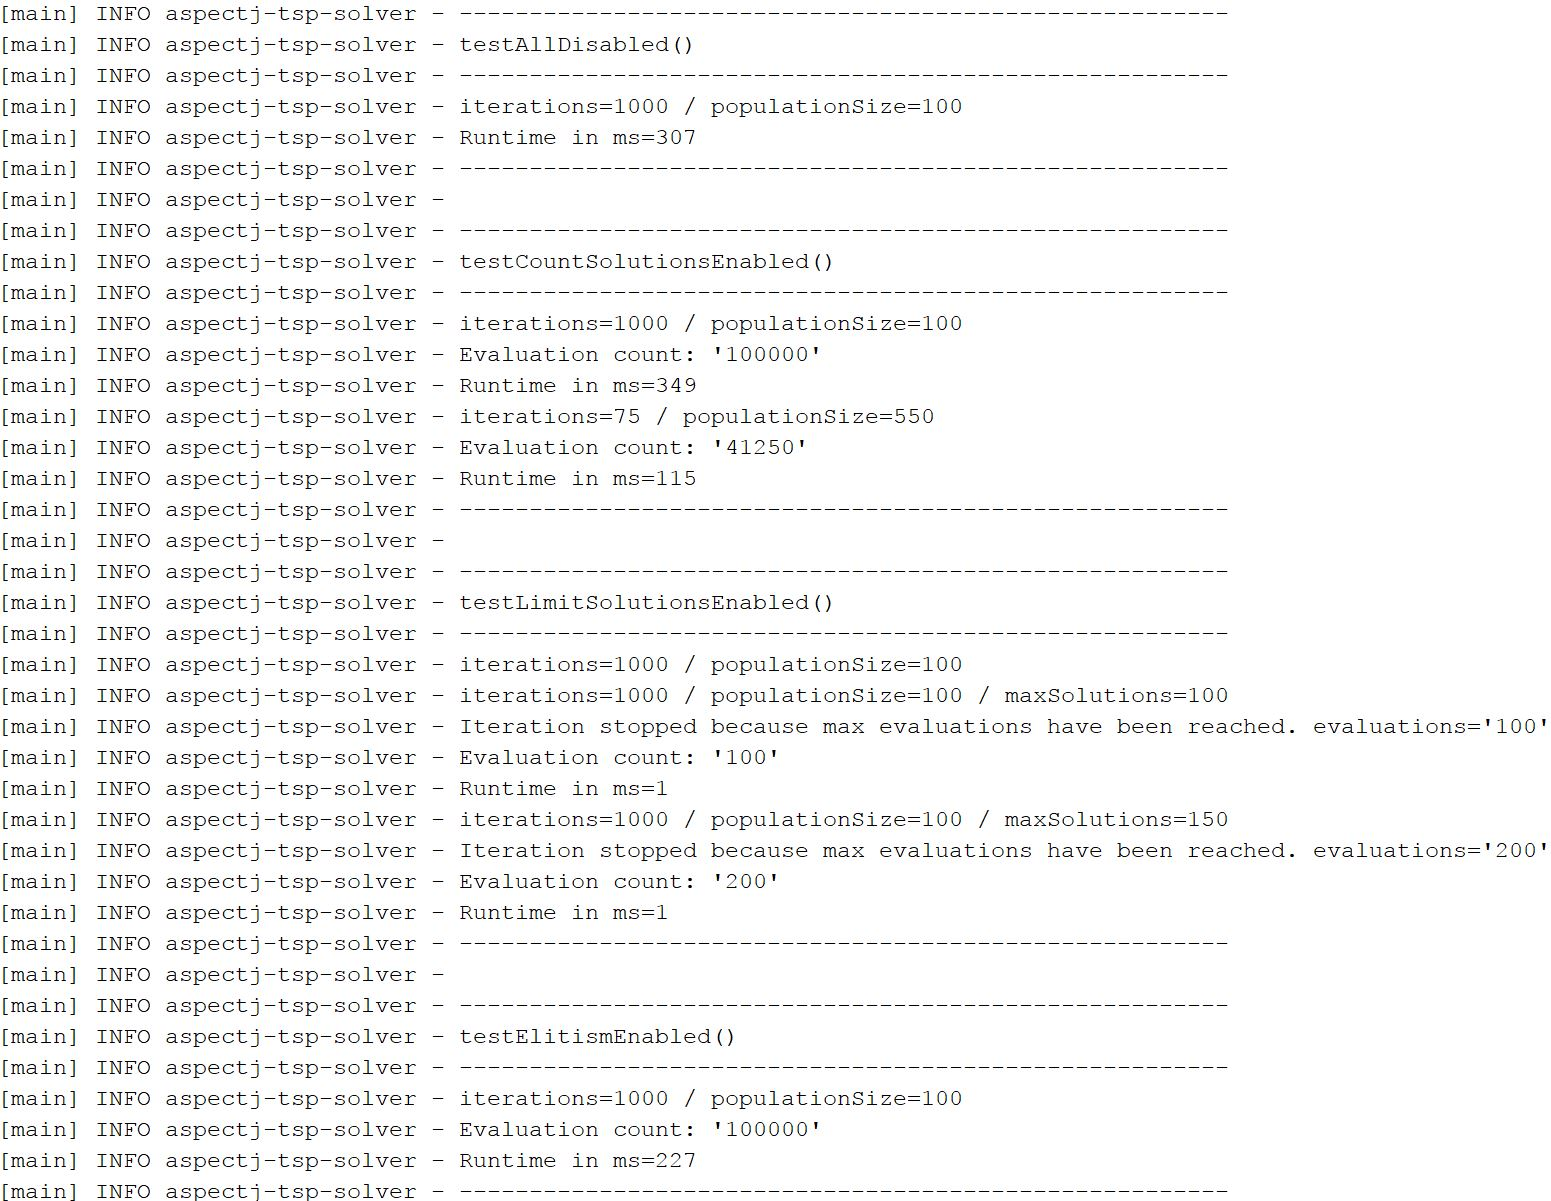
\includegraphics[scale=0.5]{\imageDir/tsp-solver-log-1.JPG}
	\caption{\emph{TSP-Solver Logs} Teil 1}
\end{figure}
\begin{figure}[h]
	\centering
	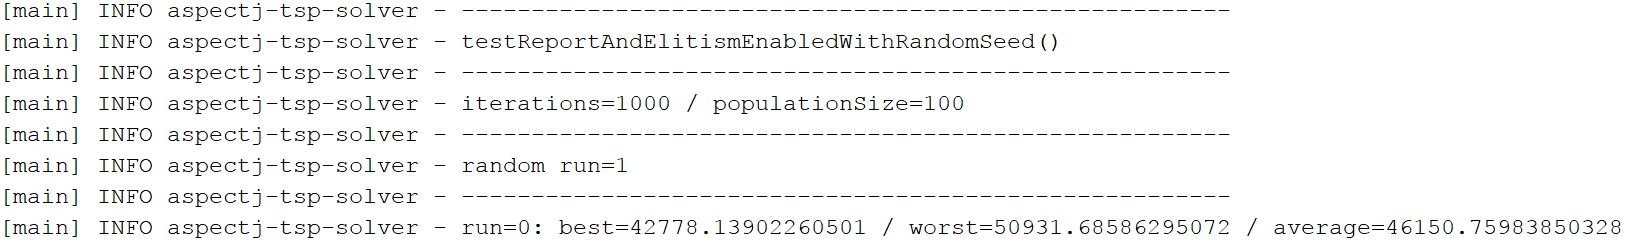
\includegraphics[scale=0.5]{\imageDir/tsp-solver-log-2.JPG}
	\caption{\emph{TSP-Solver Logs} Teil 2}
\end{figure}
\ \newpage

\begin{figure}[h]
\centering
	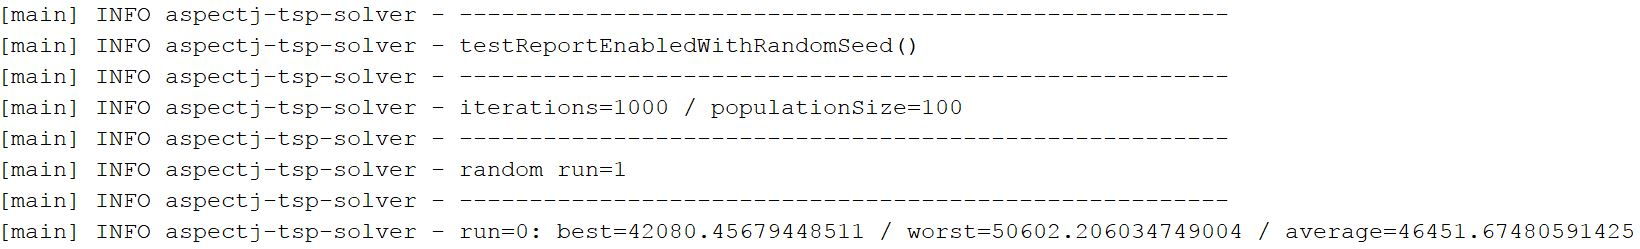
\includegraphics[scale=0.5]{\imageDir/tsp-solver-log-3.JPG}
	\caption{\emph{TSP-Solver Logs} Teil 3}
\end{figure}
\ \newline
\begin{figure}[h]
	\centering
	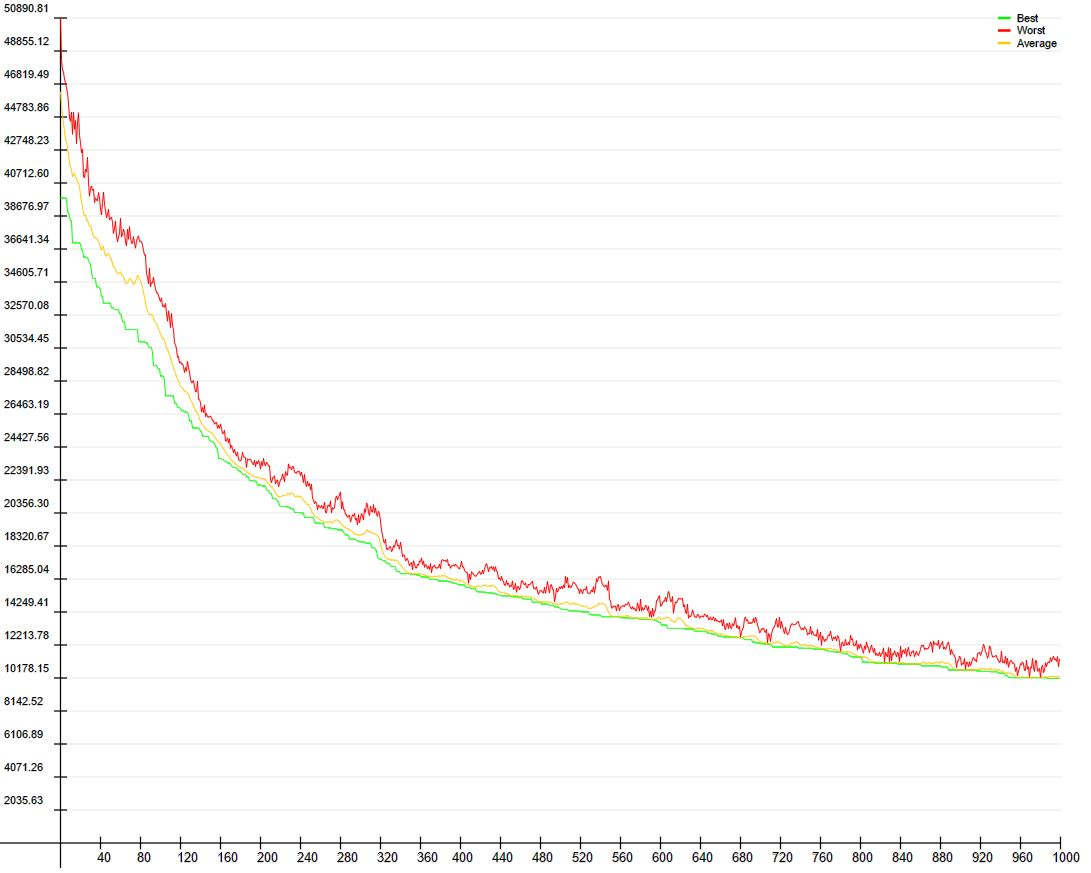
\includegraphics[scale=0.7]{\imageDir/tsp-solver-elitism-random-1.JPG}
	\caption{\emph{TSP-Solver, Random Seed, Elitism} erster Durchlauf}
\end{figure}
\ \newpage

\begin{figure}[h]
	\centering
	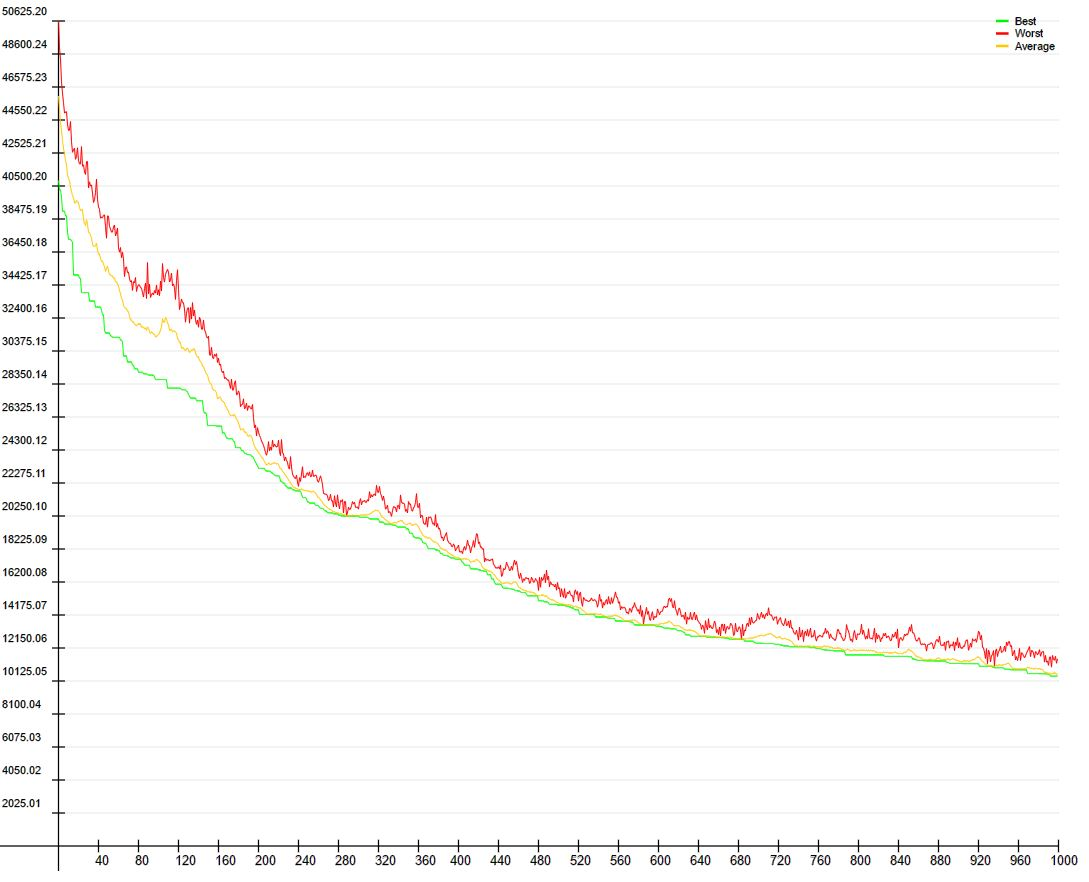
\includegraphics[scale=0.7]{\imageDir/tsp-solver-elitism-random-2.JPG}
	\caption{\emph{TSP-Solver, Random Seed, Elitism} zweiter Durchlauf}
\end{figure}
\ \newpage

\begin{figure}[h]
	\centering
	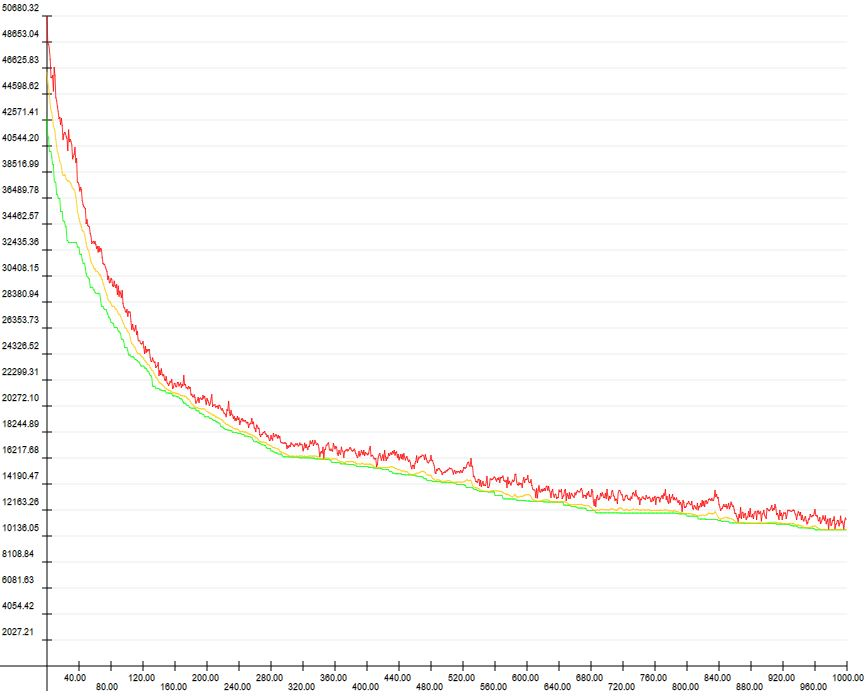
\includegraphics[scale=0.7]{\imageDir/tsp-solver-elitism-random-3.JPG}
	\caption{\emph{TSP-Solver, Random Seed, Elitism} dritter Durchlauf}
\end{figure}
\ \newpage

\begin{figure}[h]
	\centering
	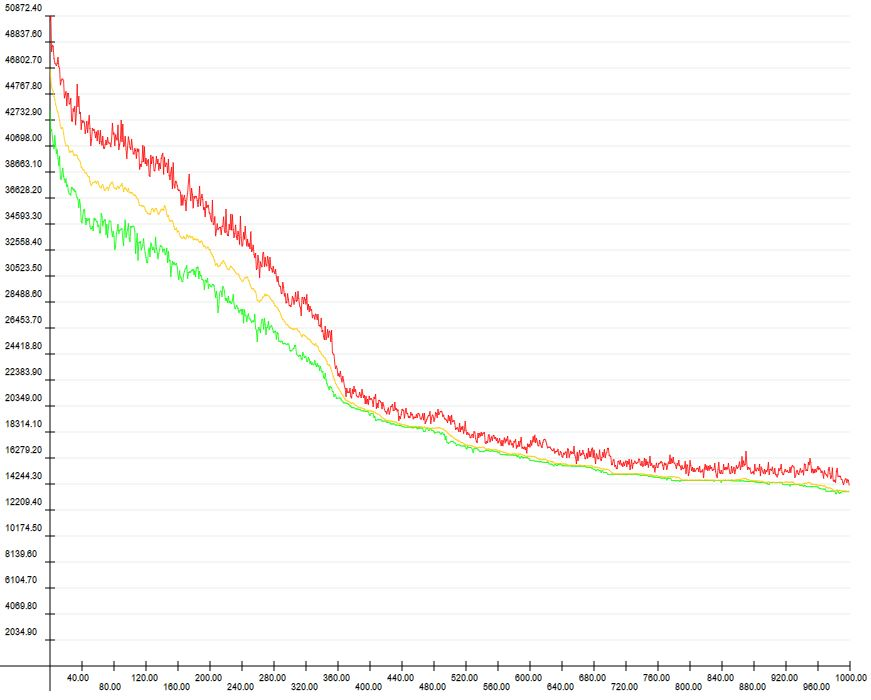
\includegraphics[scale=0.7]{\imageDir/tsp-solver-random-1.JPG}
	\caption{\emph{TSP-Solver, Random Seed} erster Durchlauf}
\end{figure}

\ \newpage
\begin{figure}[h]
	\centering
	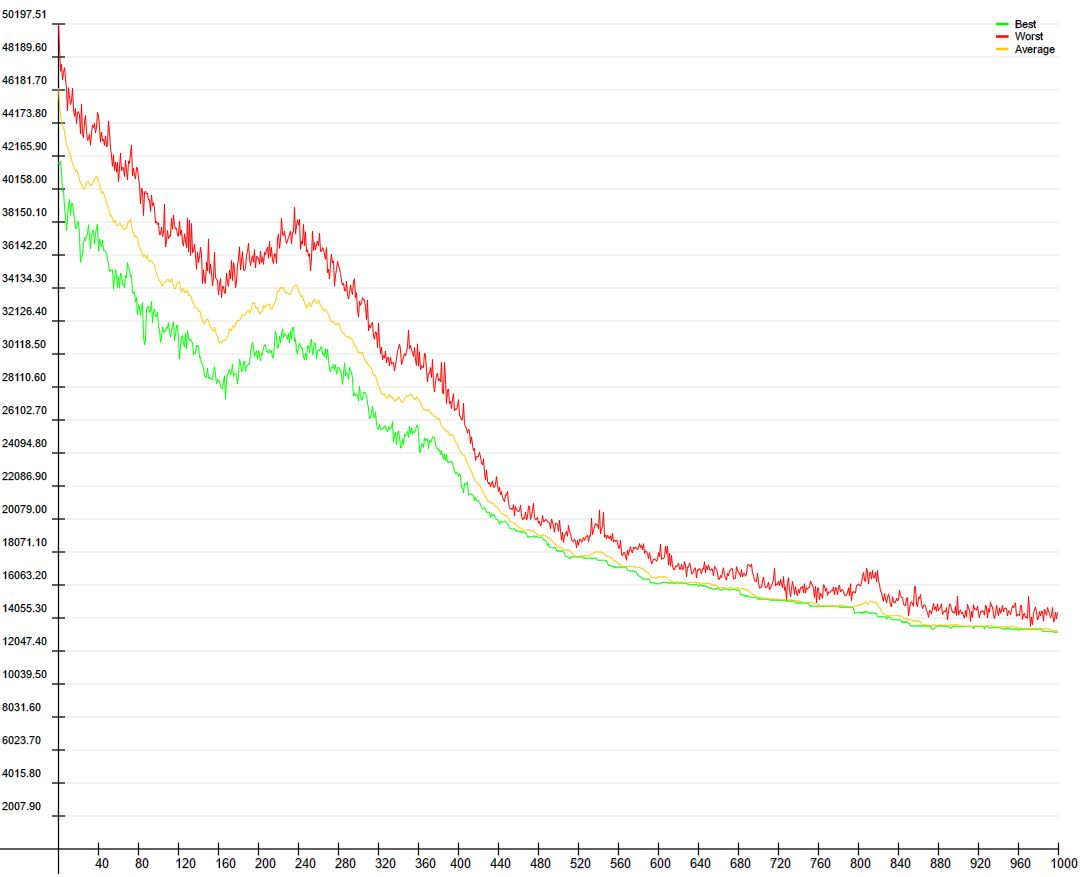
\includegraphics[scale=0.7]{\imageDir/tsp-solver-random-2.JPG}
	\caption{\emph{TSP-Solver, Random Seed} zweiter Durchlauf}
\end{figure}

\ \newpage
\begin{figure}[h]
	\centering
	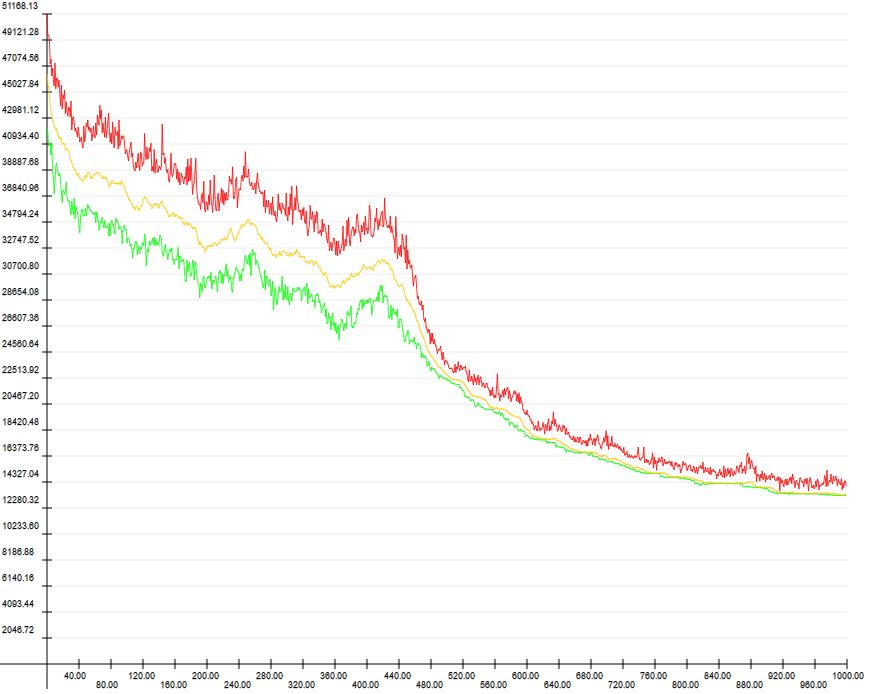
\includegraphics[scale=0.7]{\imageDir/tsp-solver-random-3.JPG}
	\caption{\emph{TSP-Solver, Random Seed} dritterDurchlauf}
\end{figure}

\end{document}